\documentclass{beamer}
%\usecolortheme{spruce}
\usetheme{A}

\usepackage{amsmath}
\usepackage{datetime}
\usepackage{relsize}
\usepackage{ulem}
\usepackage{amsmath}
\usepackage{calc}
\usepackage{tikz}
\usepackage{tabularx}
\usepackage{stmaryrd}
\usepackage{wasysym}
\usepackage{booktabs}
\usepackage{multicol}
\usepackage{colortbl}
\usepackage{proof}
\usepackage{relsize}

\usepackage{fontspec}
\newfontfamily\DejaSans{DejaVu Sans}

\definecolor{darkgreen}{HTML}{009900}
\definecolor{darkred}{HTML}{e60000}
\newcommand{\dg}[1]{\textcolor{darkgreen}{#1}}
\newcommand{\dr}[1]{\textcolor{darkred}{#1}}
\newcommand{\happy}{\dg{\smiley}}
\newcommand{\sad}{\dr{\frownie}}
\newcommand{\term}[1]{\ensuremath{\mathtt{#1}}}
\newcommand{\li}{\!\multimap\!}
\newcommand{\lotimes}{\!\otimes\!}
\newcommand{\loplus}{\!\oplus\!}
\newcommand{\lin}[1]{\langle#1\rangle}
\newcommand{\lint}[1]{[#1]}
\newcommand{\cat}[1]{\footnotesize \textsc{#1}}	
\newcommand{\W}[1]{\scriptsize #1}
\newcommand{\etext}[1]{\scriptsize {\textit{#1}}}
\newcommand{\smain}{\cat{S}$_{\text{main}}$}
\newcommand{\ssub}{\cat{S}$_{\text{sub}}$}
\newcommand{\type}[2]{\scriptsize\ensuremath{\textcolor{#2}{#1}}}
\newcommand{\red}[1]{\textcolor{red}{{}_#1}}

%{\DejaSans ☺😐☹😁😂😃😇😉😈😋😍😱}

\newcolumntype{L}{>{\raggedright\arraybackslash}X}
\newcommand{\hnorm}{\vphantom{()}}
\newcommand{\dgat}[2]{\alt<#1>{\dg{#2}}{#2}}
\newcommand{\drat}[2]{\alt<#1>{\dr{#2}}{#2}}
\newcommand{\boxat}[2]{\ensuremath{\alt<#1>{\boxed{#2}}{#2}}}
\newcommand{\qmarkat}[2]{\alt<#1>{#2}{???}}
\newcommand{\gqmarkat}[2]{\dg{\alt<#1>{#2}{???}}}
\newcommand{\rqmarkat}[2]{\dr{\alt<#1>{#2}{???}}}

\usetikzlibrary{calc}


\hypersetup{
    colorlinks=true,
    urlcolor=blue,
    pdfpagemode=FullScreen,
}


\begin{document}


\date{ESSLLI, August 2022, Galway}

\title[]{Logic-Based Parsing with Neural Networks}
\subtitle{Compositional Models of Vector-based Semantics}
\author{%
    Konstantinos Kogkalidis
    \inst{Utrecht Institute of Linguistics OTS, Utrecht University}
}

{%
\setbeamertemplate{headline}{}
\frame{\titlepage
\hspace{-10pt}
}
}

{
\setbeamercolor{background canvas}{bg=black}
\begin{frame}[plain]{}
\noindent
\centering
\larger[5]
\vfill
\textcolor{pink}{\DejaSans{☮ Certified}\\
\smaller[3]
no military applications/funding}
\end{frame}
}

\begin{frame}{The agenda}
	\smaller
	\begin{itemize}
		\item exploring \AE thel
		\item parsing with graph learning machinery
	\end{itemize}
\end{frame}


\section{Recap: Grammar}

\begin{frame}{Types}
	\smaller	
	
		ILL$_{\li}$ plus $\diamondsuit, \Box$ modalities for \textit{dependency domain demarkation}.
	\vfill
		
	$\mathbb{T}$ inductively defined as:
	\[
		\mathbb{T} := A \ 
					\uncover<2->{| \  T \li T \ 
					\uncover<3->{| \ \diamondsuit^d  T \ 
					\uncover<4->{| \ \Box^d T
					}}}
					\qquad A \in \mathbb{A}, T \in \mathbb{T}
	\]
	\vfill	

	\begin{itemize}
		\item[$\mathbb{A}$] 				-- closed set of base types
		\uncover<2->{
		\item[$\li$]						-- linear function builder
		\uncover<3->{
		\item[$\diamondsuit$] 				-- reserved for "necessary arguments", i.e. complements
		\uncover<4->{
		\item[$\Box$]						-- reserved for "optional functors", i.e. adjuncts
		}}}
	\end{itemize}
\end{frame}

\begin{frame}{Rules \& Terms}
	\smaller
	
	\renewcommand{\arraystretch}{1.15}
	\alt<5->{Bonus:
	\vfill
	\smaller
	\centering
	ad-hoc extraction
	\[
	\infer[\mathsf{X}]{\langle\Gamma, \Delta\rangle^d,  \langle \term{x}: T_1 \rangle^\mathsf{X} \vdash \term{s}: T_2}{
	\langle\Gamma, \langle \term{x}: T_1 \rangle^\mathsf{X}, \Delta\rangle^d \vdash \term{s}: T_2}
	\]
	}{
	\begin{tabularx}{\textwidth}{@{}c@{\qquad}c@{}}
	\multicolumn{2}{l}{{\DejaSans 😃} \smaller ~ function/argument structures}\\
	$\infer[Lex]{\term{c}: T \vdash \term{c}: T}	{\vphantom{T}}$
	&
	$\infer[\li E]{\Gamma, \Delta \vdash \term{s\ t}: T_2}{\Gamma \vdash \term{s}: T_1 \li T_2 & \Delta \vdash \term{t}: T_1}$
	\\
	\visible<2->{
	\\
	\multicolumn{2}{l}{{\DejaSans ☺} \smaller ~ simple dependency demarkation}\\
	$\infer[\diamondsuit^d I]{\langle \Gamma \rangle^{d} \vdash \vartriangle^d \term{t}: \diamondsuit^d T}{\Gamma \vdash \term{t}: T}$
	&
	$\infer[\Box^d E]{\langle \Gamma \rangle^d \vdash \blacktriangledown^d \term{s}: T}{\Gamma \vdash \term{s}: \Box^d T}$
	\\
	\visible<3->{
	\\
	\multicolumn{2}{l}{{\DejaSans 😐} \smaller ~ hypothetical reasoning}\\
	$\infer[Ax]{\term{x}: T \vdash \term{x}: T}	{\vphantom{T}}$
	&
	$\infer[\li I]{\Gamma \vdash \lambda\term{x.s}: T_1 \li T_2}{\Gamma, \term{x}: T_1 \vdash \term{s}: T_2}$	
	\\
	\visible<4->{
	\\
	\multicolumn{2}{l}{{\DejaSans 😱} \smaller ~ cosmic horror from the great beyond}\\
	$\infer[\Box^d I]{\Gamma \vdash \blacktriangle^d \term{s}: \Box^d T}{\langle \Gamma \rangle^d \vdash \term{s}: T}$
	&
	$\infer[\diamondsuit^d E]{\Gamma[\Delta] \vdash \term{t}[\term{x} \mapsto \triangledown^d \term{s}]: T_2}{
			\Gamma[\langle \term{x}: T_1 \rangle^d] \vdash \term{t}: T_2			
			&\quad
			\Delta \vdash \term{s}: \diamondsuit^d T_1}$
	\\
	}}}
	\end{tabularx}}
\end{frame}


\begin{frame}{Today's Example}
	alt-tab
\end{frame}


\section{Proof Nets}

\begin{frame}{\alt<13->{Formula Decomposition: Polarity Induction}{Formula Decomposition: Types $\equiv$ Trees}}

\smaller

\alt<13->
{
subtree polarity (\textit{preserved} to the right, \textit{inverted} to the left)
\begin{itemize}
	\item[+] we \dg{have}
	\item[-] we \dr{miss}
\end{itemize}
\flushright
}
{
	The type assignment of \textit{``where''}:
	\[
	\alt<2->{
		\alt<4>{\textcolor{red}{\diamondsuit ^{relcl}}}{\diamondsuit ^{relcl}}
				(\alt<6>{\textcolor{red}{!^{x}}}{!^{x}}
					\alt<7>{\textcolor{red}{!^{mod}}}{!^{mod}}
						(\alt<9>{\textcolor{red}{ppart}}{ppart}
					\alt<8>{\textcolor{red}{\multimap}}{\multimap} 
						\alt<10>{\textcolor{red}{ppart}}{ppart})
			\alt<5>{\textcolor{red}{\multimap}}{\multimap} 
				\alt<11>{\textcolor{red}{ssub}}{ssub})
	\alt<3>{\textcolor{red}{\multimap}}{\multimap} 
		\Box ^{mod}(np\multimap np)
	}
	{
	\diamondsuit ^{relcl}(\diamondsuit ^{x}\Box ^{x}\diamondsuit ^{mod}\Box ^{mod}(ppart\multimap ppart)\multimap ssub)\multimap \Box ^{mod}(np\multimap np)
	}
	\]
}
\vfill


\alt<3->{
	\smaller
	\centering
	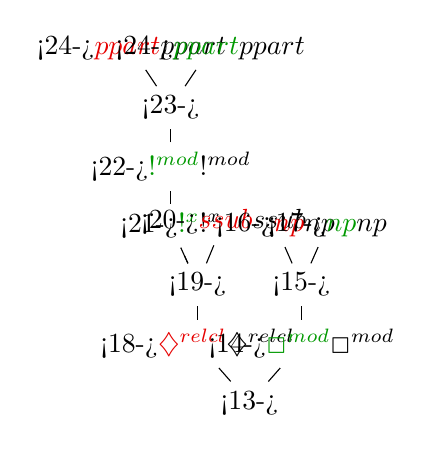
\begin{tikzpicture}
		\visible<3->{\node 		(b0)				at (0, 0)				{\dgat{13-}{$\multimap$}};
		\visible<4->{\node 		(rc)				at (-0.66, 0.75)		{\drat{18-}{$\diamondsuit^{relcl}$}};
		\draw (b0) -- (rc);
		\visible<5->{\node 		(b1)				at (-0.66, 1.5)			{\drat{19-}{$\multimap$}};
		\draw (rc) -- (b1);
		\visible<6->{\node 		(!x)				at (-1, 2.25)			{\dgat{21-}{$!^{x}$}};
		\alt<21->{
			\draw[dashed] (b1) -- (!x);
		}{
			\draw (b1) -- (!x);
		}
		\visible<7->{\node 		(!m)				at (-1, 3)				{\dgat{22-}{$!^{mod}$}};
		\draw (!x) -- (!m);
		\visible<8->{\node 		(b2)				at (-1, 3.75)			{\dgat{23-}{$\multimap$}};
		\draw (!m) -- (b2);
		\visible<9->{\node 		(pp0)				at (-1.5, 4.5)			{\drat{24-}{$ppart$}};
		\draw (b2) -- (pp0);
		\visible<10->{\node 	(pp1)				at (-0.5, 4.5)			{\dgat{24-}{$ppart$}};
		\draw (b2) -- (pp1);
		\visible<11->{\node		(ssub)				at (-0.33, 2.3)			{\hnorm \drat{20-}{$ssub$}};
		\draw (b1) -- (ssub);
		\visible<12->{
		\node 					(bm)				at (0.66, 0.75)			{\dgat{14-}{$\Box^{mod}$}};
		\draw (b0) -- (bm);
		\node					(b3)				at (0.66, 1.5)			{\dgat{15-}{$\multimap$}};
		\draw (bm) -- (b3);
		\node					(np1)				at (0.33, 2.25)			{\drat{16-}{$np$}};
		\draw (b3) -- (np1);
		\node					(np2)				at (0.99, 2.25)			{\dgat{17-}{$np$}};
		\draw (b3) -- (np2);
		}}}}}}}}}}
	\end{tikzpicture}
}
{
	\flushright
	\visible<2>{\textit{$!(\_) := \diamondsuit\Box(\_)$}}
}
\end{frame}

\begin{frame}{\alt<9->{\alt<41->{Proof \sout{\sout{Frames} Structures} Nets}{Proof \sout{Frames} Structures}}{Proof Frames}}
\smaller[2]

	\centering
	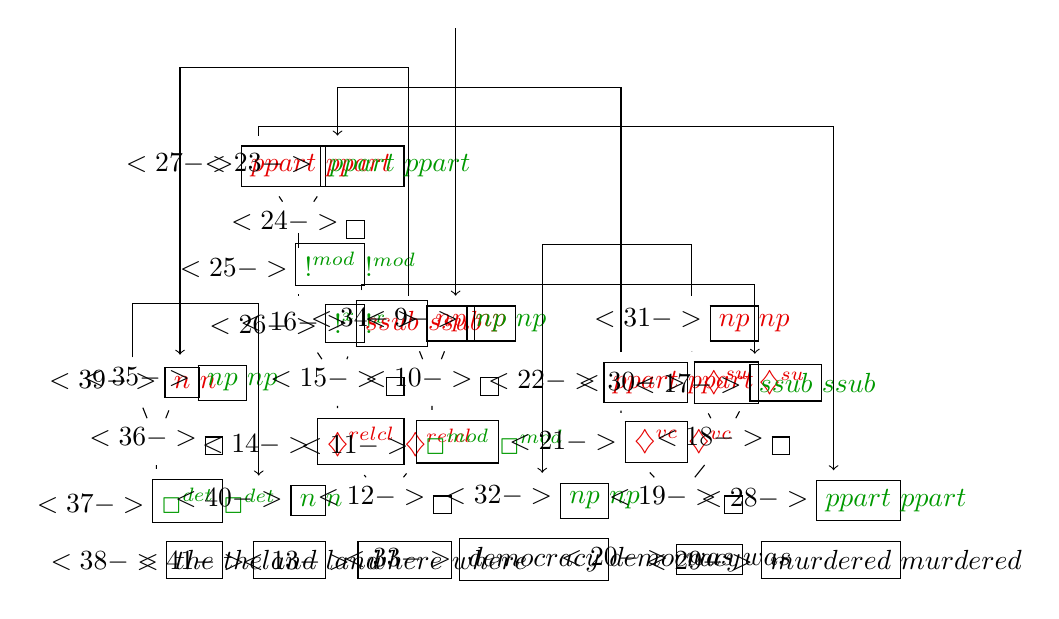
\begin{tikzpicture}
		\node 					(the)         		at (-0.3, 0)   			{\boxat{38-}{the}};
		\node 					(t1_det)         	at (-0.3, 0.75)      	{$\boxat{37-}{\dg{\Box^{det}}}$};
		\node					(t1_b0)				at (-0.3, 1.5)			{$\boxat{36-}{\dg{\multimap}}$};
		\node					(t1_n)				at (-0.6, 2.25)			{$\boxat{39-}{\dr{n}}$};
		\node					(t1_np)				at (0, 2.25)			{$\boxat{35-}{\dg{np}}$};
		\draw (t1_det) -- (t1_b0) -- (t1_n);
		\draw (t1_b0) -- (t1_np);
%		--------------------------------------------------------------------------------------------------------
		\node					(land)				at (1, 0)				{\boxat{41-}{land}};
		\node					(t2_n)				at (1, 0.75)			{$\boxat{40-}{\dg{n}}$};
%		--------------------------------------------------------------------------------------------------------
		\node					(where)				at (2.6, 0)				{\boxat{13-}{where}};		
		\node 					(t3_b0)				at (2.6, 0.75)			{$\boxat{12-}{\dg{\multimap}}$};		
		\node 					(t3_rc)				at (2.0, 1.5)			{$\boxat{14-}{\dr{\diamondsuit^{relcl}}}$};
		\node 					(t3_b1)				at (2.0, 2.25)			{$\boxat{15-}{\dr{\multimap}}$};		
		\node 					(t3_!x)				at (1.5, 3.0)			{$\boxat{26-}{\dg{!^{x}}}$};
		\node 					(t3_!m)				at (1.5, 3.75)			{$\boxat{25-}{\dg{!^{mod}}}$};		
		\node 					(t3_b2)				at (1.5, 4.25)			{$\boxat{24-}{\dg{\multimap}}$};
		\node 					(t3_p1)				at (1.0, 5.)			{$\boxat{27-}{\dr{ppart}}$};
		\node 					(t3_p2)				at (2., 5.)				{$\boxat{23-}{\dg{ppart}}$};
		\node					(t3_ss)				at (2.3, 3.0)			{$\boxat{16-}{\hnorm \dr{ssub}}$};
		\node					(t3_bm)				at (3.2, 1.5)			{$\boxat{11-}{\dg{\Box^{mod}}}$};
		\node					(t3_b3)				at (3.2, 2.25)			{$\boxat{10-}{\dg{\multimap}}$};
		\node					(t3_np1)			at (2.9, 3)				{$\boxat{34-}{\dr{np}}$};
		\node					(t3_np2)			at (3.5, 3)				{$\boxat{9-}{\dg{np}}$};
		\draw (t3_b0) -- (t3_rc) -- (t3_b1);
		\draw[dashed] (t3_b1) --  (t3_!x);
		\draw (t3_!x) -- (t3_!m) -- (t3_b2);
		\draw (t3_b2) -- (t3_p1);
		\draw (t3_b2) -- (t3_p2);
		\draw (t3_b1) -- (t3_ss);
		\draw (t3_b0) -- (t3_bm) -- (t3_b3) -- (t3_np1);
		\draw (t3_b3) -- (t3_np2);
%		--------------------------------------------------------------------------------------------------------
		\node					(democracy)			at (4.6, 0)				{\boxat{33-}{democracy}};
		\node					(t4_np)				at (4.6, 0.75)			{$\boxat{32-}{\dg{np}}$};
%		--------------------------------------------------------------------------------------------------------
		\node					(was)				at (6.3, 0)				{\boxat{20-}{was}};
		\node					(t5_b0)				at (6.3, 0.75)			{$\boxat{19-}{\dg{\multimap}}$};
		\node					(t5_vc)				at (5.6, 1.5)			{$\boxat{21-}{\dr{\diamondsuit^{vc}}}$};
		\node					(t5_pp)				at (5.6, 2.25)			{$\boxat{22-}{\dr{ppart}}$};
		\node					(t5_b1)				at (6.9, 1.5)			{$\boxat{18-}{\dg{\multimap}}$};
		\node					(t5_su)				at (6.5, 2.25)			{$\boxat{30-}{\dr{\diamondsuit^{su}}}$};
		\node					(t5_np)				at (6.5, 3)				{$\boxat{31-}{\dr{np}}$};
		\node					(t5_ss)				at (7.3, 2.25)			{$\boxat{17-}{\dg{ssub}}$};
		\draw (t5_b0) -- (t5_vc) -- (t5_pp);
		\draw (t5_b0) -- (t5_b1) -- (t5_su) -- (t5_np);
		\draw (t5_b1) -- (t5_ss);
%		--------------------------------------------------------------------------------------------------------
		\node					(murdered)			at (8.3, 0)				{\boxat{29-}{murdered}};
		\node					(t6_pp)				at (8.3, 0.75)			{$\boxat{28-}{\dg{ppart}}$};
%		--------------------------------------------------------------------------------------------------------
		AXIOM LINKS
		\visible<2->{
		\draw[->] (t1_n) -- ($(t1_n) + (0,1)$) -|  (t2_n);
		}
		\visible<3->{		
		\draw[->] (t3_np1)	-- ($(t3_np1) + (0,3.25)$) -| (t1_np);
		}
		\visible<4->{
		\draw[->] (t5_np) -- ($(t5_np) + (0,1)$) -| (t4_np);
		}
		\visible<5->{
		\draw[->] (t3_ss) -- ($(t3_ss) + (0, 0.5)$) -| (t5_ss);
		}
		\visible<6->{
		\draw[->] (t3_p1) -- ($(t3_p1) + (0,0.5)$) -| (t6_pp);
		}
		\visible<7->{
		\draw[->] (t5_pp) -- ($(t5_pp) + (0,3.75)$) -| (t3_p2);
		}
		\visible<8->{
		\draw[<-] (t3_np2) -- ($(t3_np2) + (0, 3.75)$);
		}
	\end{tikzpicture}
	
	\smaller
	\visible<9->{
	$
	\textcolor{red}{
	\alt<10->{
	\alt<11->{\blacktriangledown ^{mod}(
		\alt<12->{
			\alt<13->{\textsf{where}}{???}
			~
			\alt<14->{\vartriangle^{relcl}(\alt<15->{\lambda \mathrm{x_{0}}.(\alt<18->{\alt<19->{\alt<20->{\textsf{was}}{???}~
			\alt<21->{\vartriangle^{vc}(\alt<24->{\alt<25->{\blacktriangledown ^{mod}\triangledown ^{mod}\alt<26->{\blacktriangledown ^{x}\triangledown ^{x}\alt<27->{\mathrm{x_{0}}}{???}}{(???)}}{???}
			~\alt<29->{\textsf{murdered}}{???}}{???})}{???}}{???}
			~\alt<30->{\vartriangle^{su}\alt<33->{\textsf{democracy}}{???}}{???}}{???})}{???})}{???}}{???}
	)}{???}
	~ 
	\alt<36->{(\alt<37->{\blacktriangledown^{det}\alt<38->{\textsf{the}}{???}}{???}
	~\alt<41->{\textsf{land}}{???})}{???}}{}	
%	\blacktriangledown ^{mod}(\textsf{where}~\vartriangle ^{relcl}\lambda \mathrm{x_{0}}.(\textsf{was}~\vartriangle ^{vc}(\blacktriangledown ^{mod}\triangledown ^{mod}\blacktriangledown ^{x}\triangledown ^{x}\mathrm{x_{0}}~\textsf{murdered})~\vartriangle ^{su}\textsf{democracy}))~
%	(\blacktriangledown ^{det}\textsf{the}~\textsf{land})
	}
	$
	}
%	
\vfill
\end{frame}

{%
\setbeamercolor{background canvas}{bg=black}
\begin{frame}[plain]{}
\larger[2]
\vfill
\centering
\textcolor{teal!50}{
written and directed by\\
\textsc{kokos}
}
\vfill
\end{frame}
}

\section{Going Neural}

\begin{frame}
\flushright
\larger
\textit{``Lets neural sh!t up''}\\
\smaller
-- Alonzo Church, 1973

\vfill

\flushleft
\smaller[2]
\visible<2->{
\textit{disclaimer: not an actual quote}
}
\end{frame}


\begin{frame}{Main ingredients}
\smaller

\begin{itemize}
\item Type assignment (supertagging)\\
parallel tree decoding with dynamic graph convolutions
\item Axiom linking (neural bijections)\\
optimal transport with Sinkhorn iterations
\item Formal verification\\
proof net traversal
\end{itemize}
\end{frame}


\begin{frame}{Supertagging 101}
	\smaller
	
	\begin{block}{goal}
	maximize $p(T_1, \dots T_n)$ conditional on some input $(w_1,\dots w_n)$	
	\end{block}
	\vfill
	\pause
	\begin{block}{\alert{the catch}}
	types are sparse $\implies$ fixed vocabulary classification = no good
	\end{block}
\end{frame}


\begin{frame}{Supertagging as parallel graph completion}
	\smaller[2]
	\centering
	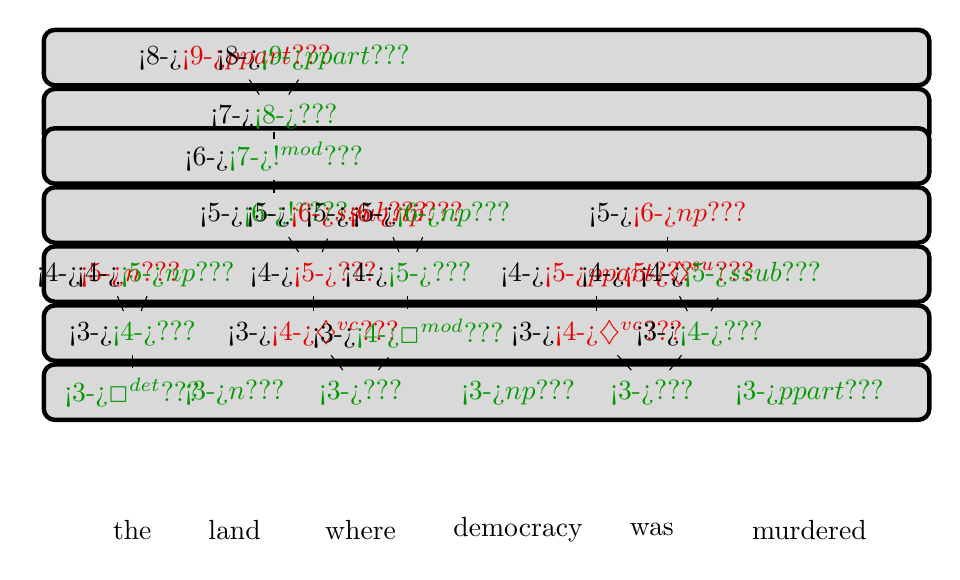
\begin{tikzpicture}
		\visible<8>{
			\node[rectangle, inner sep=0pt, minimum width=320pt, minimum height=20pt, rounded corners, ultra thick,draw=black,fill=gray!30]
			(bert)
			at
			(4.2, 5) {};
		}
		\visible<7>{
			\node[rectangle, inner sep=0pt, minimum width=320pt, minimum height=20pt, rounded corners, ultra thick,draw=black,fill=gray!30]
			(bert)
			at
			(4.2, 4.25) {};
		}
		\visible<6>{
			\node[rectangle, inner sep=0pt, minimum width=320pt, minimum height=20pt, rounded corners, ultra thick,draw=black,fill=gray!30]
			(bert)
			at
			(4.2, 3.75) {};
		}
		\visible<5>{
			\node[rectangle, inner sep=0pt, minimum width=320pt, minimum height=20pt, rounded corners, ultra thick,draw=black,fill=gray!30]
			(bert)
			at
			(4.2, 3) {};
		}
		\visible<4>{
			\node[rectangle, inner sep=0pt, minimum width=320pt, minimum height=20pt, rounded corners, ultra thick,draw=black,fill=gray!30]
			(bert)
			at
			(4.2, 2.25) {};
		}
		\visible<3>{
			\node[rectangle, inner sep=0pt, minimum width=320pt, minimum height=20pt, rounded corners, ultra thick,draw=black,fill=gray!30]
			(bert)
			at
			(4.2, 1.5) {};
		}
		\visible<2>{
			\node[rectangle, inner sep=0pt, minimum width=320pt, minimum height=20pt, rounded corners, ultra thick,draw=black,fill=gray!30]
			(bert)
			at
			(4.2, 0.75) {};
		}

		\node 					(the)         		at (-0.3, -1)   		{the};
		\node 					(t1_det)         	at (-0.3, 0.75)      	{\gqmarkat{3-}{$\Box^{det}$}};
		\node					(t1_b0)				at (-0.3, 1.5)			{\alt<3->{\gqmarkat{4-}{$\multimap$}}{}};
		\node					(t1_n)				at (-0.6, 2.25)			{\alt<4->{\rqmarkat{5-}{$n$}}{}};
		\node					(t1_np)				at (0, 2.25)			{\alt<4->{\gqmarkat{5-}{$np$}}{}};
		\visible<3->{
		\draw (t1_det) -- (t1_b0);
		\visible<4->{
		\draw (t1_b0) -- (t1_n);
		\draw (t1_b0) -- (t1_np);		
		}}
%%		--------------------------------------------------------------------------------------------------------
		\node					(land)				at (1, -1)				{land};
		\node					(t2_n)				at (1, 0.75)			{\gqmarkat{3-}{$n$}};
%%		--------------------------------------------------------------------------------------------------------
		\node					(where)				at (2.6, -1)			{where};		
		\node 					(t3_b0)				at (2.6, 0.75)			{\gqmarkat{3-}{$\multimap$}};
		\node 					(t3_rc)				at (2.0, 1.5)			{\alt<3->{\rqmarkat{4-}{$\diamondsuit^{vc}$}}{}};
		\node 					(t3_b1)				at (2.0, 2.25)			{\alt<4->{\rqmarkat{5-}{$\multimap$}}{}};
		\node 					(t3_!x)				at (1.5, 3.0)			{\alt<5->{\gqmarkat{6-}{$!^{x}$}}{}};
		\node 					(t3_!m)				at (1.5, 3.75)			{\alt<6->{\gqmarkat{7-}{$!^{mod}$}}{}};
		\node 					(t3_b2)				at (1.5, 4.25)			{\alt<7->{\gqmarkat{8-}{$\multimap$}}{}};
		\node 					(t3_p1)				at (1.0, 5.)			{\alt<8->{\rqmarkat{9-}{$ppart$}}{}};
		\node 					(t3_p2)				at (2., 5.)				{\alt<8->{\gqmarkat{9-}{$ppart$}}{}};
		\node					(t3_ss)				at (2.3, 3.0)			{\alt<5->{\rqmarkat{6-}{\hnorm $ssub$}}{}};
		\node					(t3_bm)				at (3.2, 1.5)			{\alt<3->{\gqmarkat{4-}{$\Box^{mod}$}}{}};
		\node					(t3_b3)				at (3.2, 2.25)			{\alt<4->{\gqmarkat{5-}{$\multimap$}}{}};
		\node					(t3_np1)			at (2.9, 3)				{\alt<5->{\rqmarkat{6-}{$np$}}{}};
		\node					(t3_np2)			at (3.5, 3)				{\alt<5->{\gqmarkat{6-}{$np$}}{}};
		\visible<3->{
		\draw (t3_b0) -- (t3_rc);
		\draw (t3_b0) -- (t3_bm);
		\visible<4->{
		\draw (t3_rc) -- (t3_b1);
		\draw (t3_bm) -- (t3_b3);
		\visible<5->{
		\draw (t3_b1) -- (t3_!x);
		\draw (t3_b1) -- (t3_ss);
		\draw (t3_b3) -- (t3_np1);
		\draw (t3_b3) -- (t3_np2);
		\visible<6->{
		\draw (t3_!x) -- (t3_!m);
		\visible<7->{
		\draw (t3_!m) -- (t3_b2);
		\visible<8->{
		\draw (t3_b2) -- (t3_p1);
		\draw (t3_b2) -- (t3_p2);
		}}}}}}
%%		--------------------------------------------------------------------------------------------------------
		\node					(democracy)			at (4.6, -1)			{democracy};
		\node					(t4_np)				at (4.6, 0.75)			{\gqmarkat{3-}{$np$}};
%%		--------------------------------------------------------------------------------------------------------
		\node					(was)				at (6.3, -1)			{was};
		\node					(t5_b0)				at (6.3, 0.75)			{\gqmarkat{3-}{$\multimap$}};
		\node					(t5_vc)				at (5.6, 1.5)			{\alt<3->{\rqmarkat{4-}{$\diamondsuit^{vc}$}}{}};
		\node					(t5_pp)				at (5.6, 2.25)			{\alt<4->{\rqmarkat{5-}{$ppart$}}{}};
		\node					(t5_b1)				at (6.9, 1.5)			{\alt<3->{\gqmarkat{4-}{$\multimap$}}{}};
		\node					(t5_su)				at (6.5, 2.25)			{\alt<4->{\rqmarkat{5-}{$\diamondsuit^{su}$}}{}};
		\node					(t5_np)				at (6.5, 3)				{\alt<5->{\rqmarkat{6-}{$np$}}{}};
		\node					(t5_ss)				at (7.3, 2.25)			{\alt<4->{\gqmarkat{5-}{\hnorm $ssub$}}{}};
		\visible<3->{
		\draw (t5_b0) -- (t5_vc);
		\draw (t5_b0) -- (t5_b1);
		\visible<4->{
		\draw (t5_vc) -- (t5_pp);
		\draw (t5_b1) -- (t5_su);
		\draw (t5_b1) -- (t5_ss);
		\visible<5->{
		\draw (t5_su) -- (t5_np);
		}}}
%%		--------------------------------------------------------------------------------------------------------
		\node					(murdered)			at (8.3, -1)			{murdered};
		\node					(t6_pp)				at (8.3, 0.75)			{\gqmarkat{3-}{$ppart$}};
%%		--------------------------------------------------------------------------------------------------------
	\end{tikzpicture}
\vfill
\end{frame}

\begin{frame}{Not just a gray rectangle!}
    \smaller 
    1 decoding step per tree depth; 3 message-passing rounds per step
    \begin{itemize}
        \item \textit{contextualize: states $\to$ states}\\
        \quad \alert{universal transformer encoder w/ relative weights}\\
        \quad (many-to-many, update states with neighborhood context)
        \item \textit{predict: state $\to$ nodes}\\
        \quad \alert{token classification w/ dynamic tree embeddings}\\
        \quad (one-to-many, predict fringe nodes from current state)
        \item \textit{feedback: nodes $\to$ state}\\
        \quad \alert{heterogeneous graph attention}\\
        \quad (many-to-one, update state with last predicted nodes)
    \end{itemize} 
    \vfill
    \flushright
    [\href{https://arxiv.org/abs/2203.12235}{Kogkalidis \& Moortgat, ???}]
\end{frame}

\begin{frame}{Axiom Linking}
	\smaller
	
	\alt<11->{\smiley ~ less missing edges}{\visible<3->{\frownie ~ missing edges!}}
		{\smaller
		\begin{itemize}
			\item[\alert{!}] only consider edges between atoms of the \textit{same} sign and \textit{different} polarity
			\item[\alert{!}] each atom can only be used \textit{once}
		\end{itemize}
		}

	\smaller
	\vfill
	\centering
	\begin{tikzpicture}		
		\visible<2->{
			\draw[->] (t1_n) -- ($(t1_n) + (0,1)$) -|  (t2_n);
			\draw[->] (t3_ss) -- ($(t3_ss) + (0, 0.5)$) -| (t5_ss);
		}

	    \visible<3-10>{
	   	\draw[step=0.5] (4.99,4.99) grid (6,6);
	   	\visible<4->{
	   		\invisible<5->{
	   		\node[circle, inner sep=1pt, outer sep=0pt,draw=black]		(f1) at (3, 5.75)		{$f$};
	   		\draw[dotted, ->, thick] (t3_p1) -- (1, 5.75) -- ($(f1.west)$);
	   		\draw[dotted, ->, thick] (t3_p2) -- (3, 5) -- ($(f1.south)$);
	   		\draw[dotted, ->, thick] ($(f1.east)$) -- (5, 5.75);
	   		}
			\fill[gray!20]	(5, 5.5) 	rectangle +(0.5,0.5);
			\draw[step=0.5] (4.99,4.99) grid (6,6);
	   	}
	   	\visible<5->{
	   		\invisible<6->{
		   	\node[circle, inner sep=1pt, outer sep=0pt,draw=black]		(f2) at (3.5, 5.25)		{$f$};
		   	\draw[dotted, ->, thick] (t3_p1) -- (1, 5.25) -- ($(f2.west)$);
		   	\draw[dotted, ->, thick] (t6_pp) -- (8.3, 4) -- (3.5, 4) -- ($(f2.south)$);
		   	\draw[dotted, ->, thick] ($(f2.east)$) -- (5, 5.25);
		   	}
		   	\fill[gray!30]	(5, 5) 	rectangle +(0.5,0.5);
			\draw[step=0.5] (4.99,4.99) grid (6,6);
	   	}
	   	\visible<6->{
	   		\invisible<7->{
	   		\node[circle, inner sep=1pt, outer sep=0pt,draw=black] 	(f3) at (5.6, 4) {$f$};
			\draw[dotted, ->, thick] (t3_p2) -- ($(t3_p2) + (1, 0)$) |- ($(f3.west)$);
	   		\draw[dotted, ->, thick] (t5_pp) -- ($(f3.south)$);
	   		\draw[dotted, ->, thick] ($(f3.east)$) -- ($(f3) + (1, 0)$) |- (6, 5.75);
	   		}
		   	\fill[gray!80]	(5.5, 5.5) 	rectangle +(0.5,0.5);
			\draw[step=0.5] (4.99,4.99) grid (6,6);
	   	}
	   	\visible<7->{
	   		\invisible<8->{
	   		\node[circle, inner sep=1pt, outer sep=0pt,draw=black] 	(f4) at (6.6, 4) {$f$};
	   		\draw[dotted, ->, thick] (t5_pp) |- ($(f4.west)$);
	   		\draw[dotted, ->, thick] (t6_pp) |- ($(f4.east)$);
	   		\draw[dotted, ->, thick] (f4) |- (6, 5.25);
	   		}
	   		\fill[gray!30]	(5.5, 5) 	rectangle +(0.5,0.5);
			\draw[step=0.5] (4.99,4.99) grid (6,6);
	   	}
	   	\visible<9->{
	   		\draw[->, thick] (6.1, 5.5) -- node[above]{$\mathcal{S}$} (7.4, 5.5);
	   		\fill[gray!10] (8, 5)			rectangle +(0.5, 0.5);
	   		\fill[gray!95] (8, 5.5)			rectangle +(0.5, 0.5);
	   		\fill[gray!75] (7.5, 5)			rectangle +(0.5, 0.5);
	   		\fill[gray!10] (7.5, 5.5)		rectangle +(0.5, 0.5);
	   		\draw[step=0.5] (7.49,4.99) 	grid (8.5, 6);
	    }
	    }
	    \visible<11->{
		\draw[->] (t3_p1) -- ($(t3_p1) + (0,0.5)$) -| (t6_pp);
		\draw[->] (t5_pp) -- ($(t5_pp) + (0,3.75)$) -| (t3_p2);
		}
	
		\node 					(t1_det)         	at (-0.3, 0.75)      	{\dr{$\Box^{det}$}};
		\node					(t1_b0)				at (-0.3, 1.5)			{\dg{$\multimap$}};
		\node					(t1_n)				at (-0.6, 2.25)			{\dr{$n$}};
		\node					(t1_np)				at (0, 2.25)			{\dg{$np$}};
		\draw (t1_det) -- (t1_b0);
		\draw (t1_b0) -- (t1_n);
		\draw (t1_b0) -- (t1_np);		
%%		--------------------------------------------------------------------------------------------------------
		\node					(t2_n)				at (1, 0.75)			{\dg{$n$}};
%%		--------------------------------------------------------------------------------------------------------
		\node 					(t3_b0)				at (2.6, 0.75)			{\dg{$\multimap$}};
		\node 					(t3_rc)				at (2.0, 1.5)			{\dr{$\diamondsuit^{vc}$}};
		\node 					(t3_b1)				at (2.0, 2.25)			{\dr{$\multimap$}};
		\node 					(t3_!x)				at (1.5, 3.0)			{\dg{$!^{x}$}};
		\node 					(t3_!m)				at (1.5, 3.75)			{\dg{$!^{mod}$}};
		\node 					(t3_b2)				at (1.5, 4.25)			{\dg{$\multimap$}};
		\node 					(t3_p1)				at (1.0, 5.)			{\dr{$ppart$}};
		\node 					(t3_p2)				at (2., 5.)				{\dg{$ppart$}};
		\node					(t3_ss)				at (2.3, 3.0)			{\dr{\hnorm $ssub$}};
		\node					(t3_bm)				at (3.2, 1.5)			{\dg{$\Box^{mod}$}};
		\node					(t3_b3)				at (3.2, 2.25)			{\dg{$\multimap$}};
		\node					(t3_np1)			at (2.9, 3)				{\dr{$np$}};
		\node					(t3_np2)			at (3.5, 3)				{\dg{$np$}};
		\draw (t3_b0) -- (t3_rc);
		\draw (t3_b0) -- (t3_bm);
		\draw (t3_rc) -- (t3_b1);
		\draw (t3_bm) -- (t3_b3);
		\draw (t3_b1) -- (t3_!x);
		\draw (t3_b1) -- (t3_ss);
		\draw (t3_b3) -- (t3_np1);
		\draw (t3_b3) -- (t3_np2);
		\draw (t3_!x) -- (t3_!m);
		\draw (t3_!m) -- (t3_b2);
		\draw (t3_b2) -- (t3_p1);
		\draw (t3_b2) -- (t3_p2);
%%		--------------------------------------------------------------------------------------------------------
		\node					(t4_np)				at (4.6, 0.75)			{\dg{$np$}};
%%		--------------------------------------------------------------------------------------------------------
		\node					(t5_b0)				at (6.3, 0.75)			{\dg{$\multimap$}};
		\node					(t5_vc)				at (5.6, 1.5)			{\dr{$\diamondsuit^{vc}$}};
		\node					(t5_pp)				at (5.6, 2.25)			{\dr{$ppart$}};
		\node					(t5_b1)				at (6.9, 1.5)			{\dg{$\multimap$}};
		\node					(t5_su)				at (6.5, 2.25)			{\dr{$\diamondsuit^{su}$}};
		\node					(t5_np)				at (6.5, 3)				{\dr{$np$}};
		\node					(t5_ss)				at (7.3, 2.25)			{\dg{\hnorm $ssub$}};
		\draw (t5_b0) -- (t5_vc);
		\draw (t5_b0) -- (t5_b1);
		\draw (t5_vc) -- (t5_pp);
		\draw (t5_b1) -- (t5_su);
		\draw (t5_b1) -- (t5_ss);
		\draw (t5_su) -- (t5_np);
%%		--------------------------------------------------------------------------------------------------------
		\node					(t6_pp)				at (8.3, 0.75)			{\dg{$ppart$}};
%%		--------------------------------------------------------------------------------------------------------
	\end{tikzpicture}
\end{frame}


\begin{frame}{your turn}
	break the parser!
\end{frame}


\section{Reality Check}

\begin{frame}{Reality check}
	\smaller[2]
		\begin{itemize}
			\item tagger: applicable to any CG (\dg{applied})
			\uncover<3->{
			\item parser: adaptable to any flavor of linear logic (\dg{adapted})
			\uncover<4->{
			\item proofs: plug your own semantics / apply your own morphisms (\dr{todo})
			}}
		\end{itemize}
\end{frame}

\end{document}
